\section{Discrete manifolds}
\label{sec:discrete_man}
We will remind ourselves of the definition of a classical simplicial complex, in sets. Then we will create a type that realizes the data of a complex, using pushouts.

\subsection{Abstract simplicial complexes}

\begin{mydef}
An \defemph{abstract simplicial complex \( M \) of dimension \( n \)} is an ordered list \( M\defeq[M_0,\ldots,M_n] \) consisting of a set \( M_0 \) of vertices, and for each \( 0<k\leq n \) a set \( M_k \) of subsets of \( M_0 \) of cardinality \( k+1 \), such that for any \( j<k \), any \( (j+1) \)-element subset of an element of \( M_k \) is an element of \( M_j \). The elements of \( M_k \) are called \defemph{\( k \)-faces}. A \defemph{morphism} \( f \) from \( M=[M_0,\ldots,M_m] \) to \( N=[N_0,\ldots,N_n] \) is a function on vertices \( f:M_0\to N_0 \) such that for any face of \( M \) the image under \( f \) is a face of \( N \). Denote by \( \simcomp \) the type of abstract simplicial complexes of dimension \( n \). Let \( M_{\leq k}\defeq [M_0,\ldots,M_k] \). We call \( M_{\leq k} \) the \defemph{\( k \)-skeleton} of \( M \), and it is a (\( k \)-)complex in its own right. \( M \) is automatically equipped with a chain of inclusions of the skeleta \( M_0\hookrightarrow M_{\leq 1}\hookrightarrow\cdots\hookrightarrow M_{\leq n}=M \), which are simply the inclusions of lists into longer lists.
\end{mydef}

We can imagine constructing a simplicial complex dimension by dimension with a simple procedure of taking unions. This will parallel the realization construction that follows.

\begin{mydef}
Denote by \( \Delta(n) \) the simplicial complex obtained by taking the set of all subsets of the standard \( (n+1) \)-element set \( \Delta(n)_0\defeq\{0,\ldots,n\} \). We call \( \Delta(n) \) the \defemph{complete \( n \)-simplex}. We will refer to the \( (n-1) \)-skeleton \( \Delta(n)_{\leq(n-1)} \) with the suggestive notation \( \partial \Delta(n) \).
\end{mydef}

Note that \( \Delta(n)_{(n-1)} \) has \( n+1 \) elements. For example, \( \Delta(2)_1 \) consists of the three 2-element subsets of \( \{0, 1, 2\} \). 

Given \( M=[M_0,\ldots,M_n] \) and \( k\leq n \), a face \( f_k:M_k \) is the union of \( (k+1) \) faces in \( M_{k-1} \), and so the \( k \)-skeleton is obtained from the \( (k-1) \)-skeleton by forming the following pushout of sets:
\begin{equation}
% https://q.uiver.app/#q=WzAsNCxbMSwwLCJNX2siXSxbMCwwLCJNX2tcXHRpbWVzXFxwYXJ0aWFsIFAoaykiXSxbMCwxLCJNX3tcXGxlcSAoay0xKX0iXSxbMSwxLCJNX3tcXGxlcSBrfSJdLFsxLDAsIlxcbWF0aHJte3ByfV8xIl0sWzEsMiwiYV9rIiwyXSxbMCwzXSxbMiwzXSxbMywxLCIiLDEseyJzdHlsZSI6eyJuYW1lIjoiY29ybmVyLWludmVyc2UifX1dXQ==
\begin{tikzcd}
  {M_k\times\partial \Delta(k)} & {M_k} \\
  {M_{\leq (k-1)}} & {M_{\leq k}}
  \arrow["{\mathrm{pr}_1}", from=1-1, to=1-2]
  \arrow["{a_k}"', from=1-1, to=2-1]
  \arrow[from=1-2, to=2-2]
  \arrow[from=2-1, to=2-2]
  \arrow["\ulcorner"{anchor=center, pos=0.125, rotate=180}, draw=none, from=2-2, to=1-1]
\label{eq:attach}
\end{tikzcd}
\end{equation}

where the vertical ``attach'' map \( a_k(f_k, -) \) picks out the \( k+1 \) subsets of \( f_k \).

\begin{mydef}
In an abstract simplicial complex \( M \) of dimension \( n \), the \defemph{link} of a vertex \( v \) is the \( (n-1) \)-dimensional subcomplex containing every face \( m\in M_{n-1} \) such that \( v\notin m \) and \( m\cup v \) is an \( n \)-face of \( M \).
\label{def:link}
\end{mydef}

The link is easier to understand as all the neighboring vertices of \( v \) and the subcomplex containing these. See for example Figure~\ref{fig:link}.

\begin{figure}[h]
\centering
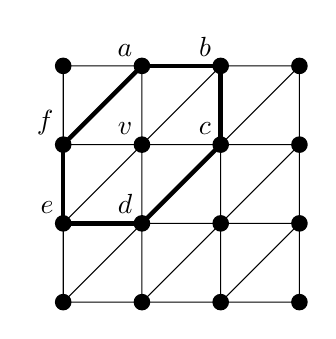
\begin{tikzpicture}
  \draw
    (0, 0) grid[step=1cm] (3, 3)
    (0, 2) edge[ultra thick] (1, 3)
    (0, 1) edge[ultra thick] (0, 2)
    (0, 1) edge[ultra thick] (1, 1)
    (1, 1) edge[ultra thick] (2, 2)
    (2, 2) edge[ultra thick] (2, 3)
    (1, 3) edge[ultra thick] (2, 3)
    (0, 1) -- (2, 3)
    (0, 0) -- (3, 3)
    (1, 0) -- (3, 2)
    (2, 0) -- (3, 1);
  \fill[radius=3pt]
    \foreach \x in {0, ..., 3} {
      \foreach \y in {0, ..., 3} {
        (\x, \y) circle[]
    }};
  \path[above left]
    \foreach \p/\v in {
      {1, 3}/a,
      {2, 3}/b,
      {0, 2}/f,
      {1, 2}/v,
      {2, 2}/c,
      {0, 1}/e,
      {1, 1}/d%
    } {
      (\p) node {$\v$}
    };
\end{tikzpicture}

\caption{The link of \( v \) in this complex consists of the vertices \( \{a,b,c,d,e,f\} \) and the edges \( \{ab,bc,cd,de,ef,fa\} \), forming a hexagon.}
\label{fig:link}
\end{figure}

\begin{mynote}
The \emph{geometric realization} of a complex uses the combinatorial data to form pushouts of standard simplices inside the category of topological spaces. A \emph{simplicial sphere} is a simplicial complex whose geometric realization is homeomorphic to a sphere. A classical 1940 result of Whitehead, building on Cairn, states that every smooth \( n \)-manifold is the geometric realization of a simplicial complex of dimension \( n \) such that the link is the geometric realization of an \( (n-1) \)-sphere\cite{whitehead_triangulation}. For more of this theory see the classic book by Kirby and Siebenmann\cite{kirby_siebenmann}.
\end{mynote}

\subsection{Higher inductive realizations}

We will realize a simplicial complex as a higher inductive type by forming a sequence of pushouts. We will work upward by dimension so as to define a standard sphere that we need in the next dimension.

\begin{mydef}
The \defemph{realization \( \mm \) of a 0-dimensional simplicial complex} \( M \) is simply the set \( M_0 \).
\end{mydef}

\begin{mydef}
The \defemph{simplicial 0-sphere} \( \bdsimplexn{1} \) is the realization of \( \partial \Delta(1) \).
\end{mydef}

\begin{mydef}
The \defemph{realization \( \mm \) of a 1-dimensional simplicial complex} \( M=[M_0, M_1] \) is the pushout
\end{mydef}
\begin{center}
% https://q.uiver.app/#q=WzAsNCxbMCwxLCJNXzA9XFxtYXRoYmJ7TX1fMCJdLFsxLDEsIlxcbWF0aGJie019XzEiXSxbMSwwLCJNXzEiXSxbMCwwLCJNXzFcXHRpbWVzIFxcYmRzaW1wbGV4bnsxfSJdLFswLDFdLFszLDAsIlxcbWF0aGJie0F9XzAiLDJdLFszLDIsIlxcbWF0aHJte3ByfV8xIl0sWzIsMSwiKl97XFxtYXRoYmJ7TX1fMX0iXSxbMSwzLCIiLDIseyJvZmZzZXQiOjMsInN0eWxlIjp7Im5hbWUiOiJjb3JuZXItaW52ZXJzZSJ9fV0sWzAsMiwiaF8xIiwyLHsic2hvcnRlbiI6eyJzb3VyY2UiOjQwLCJ0YXJnZXQiOjQwfSwibGV2ZWwiOjJ9XV0=
\begin{tikzcd}
  {M_1\times \bdsimplexn{1}} & {M_1} \\
  {M_0=\mathbb{M}_0} & {\mathbb{M}_1}
  \arrow["{\mathrm{pr}_1}", from=1-1, to=1-2]
  \arrow["{\mathbb{A}_0}"', from=1-1, to=2-1]
  \arrow["{*_{\mathbb{M}_1}}", from=1-2, to=2-2]
  \arrow["{h_1}"', shorten <=14pt, shorten >=14pt, Rightarrow, from=2-1, to=1-2]
  \arrow[from=2-1, to=2-2]
  \arrow["\ulcorner"{pos=0, rotate=180}, shift left=1, draw=none, from=2-2, to=1-1]
\end{tikzcd}
\end{center}
where \( a_k \) is the attachment data of the edges in \( M_1 \), as in diagram~\ref{eq:attach}. The right vertical map \( *_{\mm_1} \) provides a hub point for each edge, and the homotopy \( h_1 \) provides the spokes that connect the hub to the vertices.

\begin{mydef}
The \defemph{simplicial 1-sphere} \( \bdsimplexn{2} \) is the realization of \( \partial \Delta(2) \).
\end{mydef}
\begin{center}% https://q.uiver.app/#q=WzAsNCxbMCwxLCJQKDIpXzAiXSxbMSwxLCJcXHBhcnRpYWwgXFxEZWx0YV4yIl0sWzEsMCwiXFxwYXJ0aWFsIFAoMikiXSxbMCwwLCJcXHBhcnRpYWwgUCgyKVxcdGltZXMgXFxwYXJ0aWFsIFxcRGVsdGFeMSJdLFswLDFdLFszLDAsIlxcbWF0aGJie0F9XzAiLDJdLFszLDIsIlxcbWF0aHJte3ByfV8xIl0sWzIsMSwiKl97XFxwYXJ0aWFsXFxEZWx0YV4yfSJdLFsxLDMsIiIsMix7InN0eWxlIjp7Im5hbWUiOiJjb3JuZXItaW52ZXJzZSJ9fV0sWzAsMiwiaF8xIiwyLHsic2hvcnRlbiI6eyJzb3VyY2UiOjQwLCJ0YXJnZXQiOjQwfSwibGV2ZWwiOjJ9XV0=
\begin{tikzcd}
  {\partial \Delta(2)\times \bdsimplexn{1}} & {\partial \Delta(2)} \\
  {\Delta(2)_0} & {\bdsimplex{2}}
  \arrow["{\mathrm{pr}_1}", from=1-1, to=1-2]
  \arrow["{\mathbb{A}_0}"', from=1-1, to=2-1]
  \arrow["{*_{\bdsimplexn{2}}}", from=1-2, to=2-2]
  \arrow["{h_1}"', shorten <=11pt, shorten >=11pt, Rightarrow, from=2-1, to=1-2]
  \arrow[from=2-1, to=2-2]
  \arrow["\ulcorner"{anchor=center, pos=0.125, rotate=180}, draw=none, from=2-2, to=1-1]
\end{tikzcd}
\end{center}

\begin{mydef}
A \defemph{realization \( \mm \) of a 2-dimensional simplicial complex} \( [M_0, M_1, M_2] \) is the pushout
\end{mydef}
\begin{center}
% https://q.uiver.app/#q=WzAsNyxbMCwyLCJNXzFcXHRpbWVzIFxcYmRzaW1wbGV4bnsxfSJdLFswLDEsIlxcbWF0aGJie019XzAiXSxbMSwxLCJcXG1hdGhiYntNfV8xIl0sWzEsMiwiTV8xIl0sWzEsMCwiTV8yXFx0aW1lcyBcXGJkc2ltcGxleG57Mn0iXSxbMiwwLCJNXzIiXSxbMiwxLCJcXG1hdGhiYntNfV8yIl0sWzAsMSwiXFxtYXRoYmJ7QX1fMCJdLFsxLDJdLFswLDMsIlxcbWF0aHJte3ByfV8xIiwyXSxbMywyLCIqX3tcXG1hdGhiYntNfV8xfSIsMl0sWzIsMCwiIiwxLHsic3R5bGUiOnsibmFtZSI6ImNvcm5lci1pbnZlcnNlIn19XSxbMiw2XSxbNCwyLCJcXG1hdGhiYntBfV8xIiwyXSxbNSw2LCIqX3tcXG1hdGhiYntNfV8yfSJdLFs0LDUsIlxcbWF0aHJte3ByfV8xIl0sWzYsNCwiIiwxLHsic3R5bGUiOnsibmFtZSI6ImNvcm5lci1pbnZlcnNlIn19XSxbMiw1LCJoXzIiLDAseyJzaG9ydGVuIjp7InNvdXJjZSI6NDAsInRhcmdldCI6NDB9LCJsZXZlbCI6Mn1dLFsxLDMsImhfMSIsMix7InNob3J0ZW4iOnsic291cmNlIjo0MCwidGFyZ2V0Ijo0MH0sImxldmVsIjoyfV1d
\begin{tikzcd}
  & {M_2\times \bdsimplexn{2}} & {M_2} \\
  {\mathbb{M}_0} & {\mathbb{M}_1} & {\mathbb{M}_2} \\
  {M_1\times \bdsimplexn{1}} & {M_1}
  \arrow["{\mathrm{pr}_1}", from=1-2, to=1-3]
  \arrow["{\mathbb{A}_1}"', from=1-2, to=2-2]
  \arrow["{*_{\mathbb{M}_2}}", from=1-3, to=2-3]
  \arrow[from=2-1, to=2-2]
  \arrow["{h_1}"', shorten <=27pt, shorten >=27pt, Rightarrow, from=2-1, to=3-2]
  \arrow["{h_2}", shorten <=17pt, shorten >=17pt, Rightarrow, from=2-2, to=1-3]
  \arrow[from=2-2, to=2-3]
  \arrow["\ulcorner"{anchor=center, pos=0.125, rotate=-135}, draw=none, from=2-2, to=3-1]
  \arrow["\ulcorner"{anchor=center, pos=0.125, rotate=180}, draw=none, from=2-3, to=1-2]
  \arrow["{\mathbb{A}_0}", from=3-1, to=2-1]
  \arrow["{\mathrm{pr}_1}"', from=3-1, to=3-2]
  \arrow["{*_{\mathbb{M}_1}}"', from=3-2, to=2-2]
\end{tikzcd}

\end{center}
where \( \aaa_1 \) is such that this additional diagram commutes
\begin{center}
% https://q.uiver.app/#q=WzAsNCxbMSwwLCJNXzJcXHRpbWVzXFxwYXJ0aWFsXFxEZWx0YV4yIl0sWzEsMSwiXFxtYXRoYmJ7TX1fMSJdLFswLDAsIk1fMlxcdGltZXNcXHBhcnRpYWwgUCgyKSJdLFswLDEsIk1fe1xcbGVxIDF9Il0sWzAsMSwiXFxtYXRoYmJ7QX1fMSJdLFsyLDAsIlxcbWF0aHJte2lkfVxcdGltZXMgKl97XFxwYXJ0aWFsXFxEZWx0YV4yfSJdLFszLDEsIipfe1xcbWF0aGJie019X3tcXGxlcSAxfX0iLDJdLFsyLDMsImFfMSIsMl1d
\begin{tikzcd}
  {M_2\times\partial \Delta(2)} & {M_2\times\bdsimplexn{2}} \\
  {M_{\leq 1}} & {\mathbb{M}_1}
  \arrow["{\mathrm{id}\times *_{\bdsimplexn{2}}}", from=1-1, to=1-2]
  \arrow["{a_1}"', from=1-1, to=2-1]
  \arrow["{\mathbb{A}_1}", from=1-2, to=2-2]
  \arrow["{*_{\mathbb{M}_{\leq 1}}}"', from=2-1, to=2-2]
\end{tikzcd}
\end{center}
In this diagram \( a_1 \) is the simplicial attaching map from \ref{eq:attach}, and \( *_{\mathbb{M}_{\leq 1}} \) simply gathers the hub maps from \( M_0 \) and \( M_1 \) into \( \mm_1 \). The commutativity then says that \( \aaa_1 \) reflects the attachment data.
\begin{mydef}
Given a notion of realization in dimension \( n-1 \), a \defemph{realization \( \mm \) of an \( n \)-dimensional simplicial complex} \( M=[M_0, \ldots, M_n] \) is the pushout
\end{mydef}
\begin{center}%
% https://q.uiver.app/#q=WzAsMTAsWzIsMSwiXFxtYXRoYmJ7TX1fe24tMX0iXSxbMiwwLCJNX25cXHRpbWVzIFxccGFydGlhbFxcRGVsdGFebiJdLFszLDAsIk1fbiJdLFszLDEsIlxcbWF0aGJie019X24iXSxbMSwxLCJcXG1hdGhiYntNfV97bi0yfSJdLFsxLDAsIk1fe24tMn0iXSxbMiwyLCJNX3tuLTF9Il0sWzEsMiwiXFxjZG90cyJdLFswLDAsIlxcY2RvdHMiXSxbMCwxLCJcXGNkb3RzIl0sWzAsM10sWzEsMCwiXFxtYXRoYmJ7QX1fe24tMX0iLDJdLFsyLDMsIipfe1xcbWF0aGJie019X3tufX0iXSxbMSwyLCJcXG1hdGhybXtwcn1fMSJdLFszLDEsIiIsMSx7InN0eWxlIjp7Im5hbWUiOiJjb3JuZXItaW52ZXJzZSJ9fV0sWzAsMiwiaF9uIiwwLHsic2hvcnRlbiI6eyJzb3VyY2UiOjQwLCJ0YXJnZXQiOjQwfSwibGV2ZWwiOjJ9XSxbNCwwXSxbNSw0LCIqX3tcXG1hdGhiYntNfV97bi0yfX0iXSxbNiwwLCIqX3tcXG1hdGhiYntNfV97bi0xfX0iLDJdLFs4LDVdLFs5LDRdLFs3LDZdLFswLDcsIiIsMix7InN0eWxlIjp7Im5hbWUiOiJjb3JuZXItaW52ZXJzZSJ9fV0sWzQsOCwiIiwyLHsic3R5bGUiOnsibmFtZSI6ImNvcm5lci1pbnZlcnNlIn19XSxbOSw1LCJoX3tuLTJ9IiwwLHsic2hvcnRlbiI6eyJzb3VyY2UiOjQwLCJ0YXJnZXQiOjQwfSwibGV2ZWwiOjJ9XSxbNCw2LCJoX3tuLTF9IiwyLHsic2hvcnRlbiI6eyJzb3VyY2UiOjQwLCJ0YXJnZXQiOjQwfSwibGV2ZWwiOjJ9XV0=
\begin{tikzcd}
  \cdots & {M_{n-2}} & {M_n\times \bdsimplexn{n}} & {M_n} \\
  \cdots & {\mathbb{M}_{n-2}} & {\mathbb{M}_{n-1}} & {\mathbb{M}_n} \\
  & \cdots & {M_{n-1}}
  \arrow[from=1-1, to=1-2]
  \arrow["{*_{\mathbb{M}_{n-2}}}", from=1-2, to=2-2]
  \arrow["{\mathrm{pr}_1}", from=1-3, to=1-4]
  \arrow["{\mathbb{A}_{n-1}}"', from=1-3, to=2-3]
  \arrow["{*_{\mathbb{M}_{n}}}", from=1-4, to=2-4]
  \arrow["{h_{n-2}}", shorten <=8pt, shorten >=8pt, Rightarrow, from=2-1, to=1-2]
  \arrow[from=2-1, to=2-2]
  \arrow["\ulcorner"{anchor=center, pos=0.125, rotate=180}, draw=none, from=2-2, to=1-1]
  \arrow[from=2-2, to=2-3]
  \arrow["{h_{n-1}}"', shorten <=10pt, shorten >=10pt, Rightarrow, from=2-2, to=3-3]
  \arrow["{h_n}", shorten <=10pt, shorten >=10pt, Rightarrow, from=2-3, to=1-4]
  \arrow[from=2-3, to=2-4]
  \arrow["\ulcorner"{anchor=center, pos=0.125, rotate=-90}, draw=none, from=2-3, to=3-2]
  \arrow["\ulcorner"{anchor=center, pos=0.125, rotate=180}, draw=none, from=2-4, to=1-3]
  \arrow[from=3-2, to=3-3]
  \arrow["{*_{\mathbb{M}_{n-1}}}"', from=3-3, to=2-3]
\end{tikzcd}
\end{center}
where \( \aaa_n \) is such that the following commutes
\begin{center}
% https://q.uiver.app/#q=WzAsNCxbMSwwLCJNX25cXHRpbWVzXFxwYXJ0aWFsXFxEZWx0YV5uIl0sWzEsMSwiXFxtYXRoYmJ7TX1fbiJdLFswLDAsIk1fblxcdGltZXNcXHBhcnRpYWwgUChuKSJdLFswLDEsIk1fe1xcbGVxIG59Il0sWzAsMSwiXFxtYXRoYmJ7QX1fbiJdLFsyLDAsIlxcbWF0aHJte2lkfVxcdGltZXMgKl97XFxwYXJ0aWFsXFxEZWx0YV5ufSJdLFszLDEsIipfe1xcbWF0aGJie019X3tcXGxlcSBufX0iLDJdLFsyLDMsImFfMSIsMl1d
\begin{tikzcd}
  {M_n\times\partial \Delta(n)} & {M_n\times\bdsimplexn{n}} \\
  {M_{\leq n}} & {\mathbb{M}_n}
  \arrow["{\mathrm{id}\times *_{\bdsimplexn{n}}}", from=1-1, to=1-2]
  \arrow["{a_1}"', from=1-1, to=2-1]
  \arrow["{\mathbb{A}_n}", from=1-2, to=2-2]
  \arrow["{*_{\mathbb{M}_{\leq n}}}"', from=2-1, to=2-2]
\end{tikzcd}
\end{center}
Gathering some of the inductive process into one definition, we have
\begin{mydef}
\label{def:higher_realization} 
A \defemph{realization} \( \mm \) of an abstract simplicial complex \( M:\simcomp \) consists of 
\begin{enumerate}
\item \( n+1 \) types \( \mm_0,\ldots,\mm_n \) where \( \mm_0\defeq M_0 \),
\item \( n \) spans \( \myspan{\mm_{i}}{M_{i+1}\times \bdsimplexn{i+1}}{M_{i+1}}{\aaa_{i}}{\pr_1} \), \( i=0,\ldots,n-1 \), where \( \bdsimplexn{i+1} \) is the realization of the boundary of a standard simplex and \( \aaa_i \) are called \defemph{attachment maps},
\item \( n \) pushout squares from each span to \( \mm_{i+1} \), with induced maps \( \imath_i:\mm_i\to\mm_{i+1} \), \( *_{\mm_{i+1}}:M_{i+1}\to\mm_{i+1} \) and proof of commutativity \( h_{i+1} \).
\end{enumerate}
A \defemph{cellular type} \( \mm \) is a sequence of types \( \mm_0\xrightarrow[]{\imath_0}\mm_1\xrightarrow[]{\imath_1}\cdots\xrightarrow[]{\imath_{n-1}}\mm_n \), together with a proof of existence of some simplicial complex \( M \) and a realization inducing this sequence.
\end{mydef}

\subsection{Polygons}
\label{sec:polygons}

The 1-type \( \bdsimplexn{2} \) has three vertices. In order to define the link of an arbitrary realization, we will need to have \( n \)-gons for \( n\geq 3 \). For example in Figure~\ref{fig:link} the link is a 6-gon. And since \( S^1 \) could be called a 1-gon, we will also define a 1-gon, and for completeness a 2-gon.

\begin{mydef}
Define \( C(n) \), \( n\geq 3 \) to be a simplicial complex with \( C(n)_{0}=\{v_1, \ldots, v_n\} \) and edges \[ C(n)_1=\{e_1=\{v_1,v_2\}, \ldots, e_{n-1}=\{v_{n-1}, v_n\}, e_n=\{v_n, v_0\}\}. \] We call \( C(n) \) a \defemph{polygon} or \defemph{\( n \)-gon}. The realization of \( C(n) \) will be denoted \( \ccc(n) \). When it is convenient we may refer to an \( n \)-gon by \( \gr{v_1\cdots v_n} \) and to its realization by \( \hgr{v_1\cdots v_n} \).
\end{mydef}

We also have two special polygons:
\begin{mydef}
The higher inductive type \( \so \), also denoted \( \ccc(1) \), has constructors:
\begin{align*}
\so &:\Type \\
\mathsf{base}&:\so \\
\mathsf{loop}&:\mathsf{base}=\mathsf{base}
\end{align*}
\end{mydef}

\begin{mydef}
The higher inductive type \(\ccc(2) \) has constructors:
\begin{align*}
\ccc(2) &:\Type \\
v_1, v_2&:\ccc(2) \\
\ell_{12}, r_{21}&:v_1=v_2\\
\end{align*}
\end{mydef}

\begin{mylemma}\label{lem:addpoints}
\( \ccc(2)\simeq \ccc(1) \) and in fact \( \ccc(n)\simeq \ccc(n-1) \).
\end{mylemma}
\begin{myproofnonqed}
(Compare to \cite{hottbook} Lemma 6.5.1.)
\end{myproofnonqed}
First we will define \( f:\ccc(2)\to \ccc(1) \) and \( g:\ccc(1)\to \ccc(2) \), then prove they are inverses.
\begin{align*}
f(v_1)=f(v_2)&=\base &\quad g(\base)&=v_1\\
f(\ell_{12})&=\loopo&\quad g(\loopo)&=\ell_{12}\cdot r_{21}\\
f(r_{21}) &= \refl_{\base}& & \\
\end{align*}

We need to show that \( f\circ g\sim \id_{\ccc(1)} \) and \( g\circ f\sim\id_{\ccc(2)} \).
Think of \( f \) as sliding \( v_2 \) and \( v_1 \) towards each other along \( r_{21} \) coalescing into just \( v_1 \), as in Figure~\ref{fig:shrink}. This may help understand why the somewhat intricate proof is working.

\begin{figure}[h]
\centering
\begin{tikzpicture}
\tikzset{arrow/.style={-{Stealth[scale=1.1]}}}
\tikzset{oo/.style={circle, scale=0.25, fill=black}}
\tikzset{ooo/.style={circle, scale=0.25, fill=none}}
\node[oo, label=above:\( v_1 \)] (V1) at (0, 2) {};
\node[oo, label=below:\( v_2 \)] (V2) at (0, 0) {};
\node[ooo] (V21) at (0.3, 1.75) {};
\node[ooo] (V22) at (0.3, 0.25) {};
\draw (V1) edge[bend right=60, swap, "\( \ell_{12} \)"] (V2);
\draw (V1) edge[bend left=60, "\( r_{21} \)"] (V2);
\draw[arrow] (V1) edge[bend left=5] (V21);
\draw[arrow] (V2) edge[bend right=5] (V22);
\end{tikzpicture}
\caption{We imagine shrinking \( r_{21} \) down to become \( \refl_\base \) in \( S^1 \).}
\label{fig:shrink}
\end{figure}

We need terms \( p:\pit{a:\ccc(1)}f(g(a))=a \) and \( q:\pit{a:\ccc(2)}g(f(a))=a \). We will proceed by induction, defining appropriate paths on point constructors and then checking a condition on path constructors that confirms that the built-in transport of these type families respects the definition on points.

Looking first at \( g\circ f \), which shrinks \( r_{21} \), we have the following data to work with:
\begin{align*}
g(f(v_1))=g(f(v_2))&=v_1\\
g(f(\ell_{12}))&=\ell_{12}\cdot r_{21}\\
g(f(r_{21})) &= \refl_{v_1}.
\end{align*}
We then need to supply a homotopy from this data to \( \id_{\ccc(2)} \), which consists of a section and pathovers over \( \ccc(2) \):
\begin{align*}
p_1&:g(f(v_1))=v_1\\
p_2&:g(f(v_1))=v_2\\
H_\ell&:\tr(\ell_{12})(p_1)=p_2\\
H_r&:\tr(r_{21})(p_2)=p_1.
\end{align*}
which simplifies to
\begin{align*}
p_1&:v_1=v_1\\
p_2&:v_1=v_2\\
H_\ell&:g(f(\ell_{12}))^{-1}\cdot p_1\cdot \ell_{12}=p_2\\
H_r&:=g(f(r_{21}))^{-1}\cdot p_2\cdot r_{21}= p_1
\end{align*}
and then to 
\begin{align*}
p_1&:v_1=v_1\\
p_2&:v_1=v_2\\
H_\ell&:(\ell_{12}\cdot r_{21})^{-1}\cdot p_1\cdot \ell_{12}=p_2\\
H_r&:\refl_{v_1}\cdot p_2\cdot r_{21}= p_1
\end{align*}

To solve all of these constraints we can choose \( p_1\defeq\refl_{v_1} \), which by consulting either \( H_\ell \) or \( H_r \) requires that we take \( p_2\defeq{r_{21}}^{-1}\).

Now examining \( f\circ g \), we have
\begin{align*}
f(g(\base))&=\base&\\
f(g(\loopo))&=f(\ell_{12}\cdot r_{21})=\loopo
\end{align*}
and so we have an easy proof that this is the identity.

The proof of the more general case \( \ccc(n) \simeq \ccc(n-1)\) is very similar. Take the maps \( f:\ccc(n)\to \ccc(n-1) \), \( g:\ccc(n-1)\to \ccc(n) \) to be
\begin{align*}
f(v_i)=v_i&\quad(i=1,\ldots,n-1) & g(v_i)&=v_i&\quad(i=1,\ldots,n-1)\\
f(v_n)=v_1&\quad& g(e_{i,i+1})&=e_{i,i+1}&\quad(i=1,\ldots,n-2)\\
f(e_{i,i+1})=e_{i,i+1}&\quad(i=1,\ldots,n-1)& g(e_{n-1,1})&=e_{n-1,n}\cdot e_{n,1}&\\
f(e_{n-1,n})=e_{n-1,1}&&&&\\
f(e_{n,1})=\refl_{v_1}&&&&
\end{align*}
where \( f \) should be thought of as shrinking \( e_{n,1} \) so that \( v_n \) coalesces into \( v_1 \).

The proof that \( g\circ f\sim\id_{\ccc(n)} \) proceeds as follows: the composition is definitionally the identity except 
\begin{align*}
g(f(v_n))&=v_1\\
g(f(e_{n-1,n}))&=e_{n-1,n}\cdot e_{n,1}\\
g(f(e_{n,1}))&= \refl_{v_1}.
\end{align*}
Guided by our previous experience we choose \( {e_{n,1}}^{-1}:g(f(v_n))=v_n \), and define the pathovers by transport.

The proof that \( f\circ g\sim\id_{\ccc(n-1)} \) requires only noting that \( f(g(e_{n-1,1}))=f(e_{n-1,n}\cdot e_{n,1})=e_{n-1,1}\cdot\refl_{v_1}=e_{n-1,1} \).\qed

\begin{mycor}
\label{cor:gon}
All polygons are equivalent to \( \so \), i.e. we have terms \( e_n:\ccc(n)=S^1 \), and hence we have constructed a map from the unit type \( (\ccc(n), ||e_n||_{-1}):\unit\to \EMzo \).
\end{mycor}
\begin{myproof}
The proofs in Lemma~\ref{lem:addpoints} can be concatenated to give \( \ccc(n)\to\ccc(n-1)\to\cdots\to\ccc(2)\to S^1 \).
\end{myproof}

\begin{mydef}
\label{def:rotation}
Let \( R:\gr{v_1\cdots v_n}\to \gr{v_1\cdots v_n} \) (for ``rotation'') be the map sending \( v_i\mapsto v_{i+1} \) and \( v_n\mapsto v_0 \). This map clearly sends edges to edges, and so is a map of simplicial complexes, and extends to a map \( \hgr{R}:\hgr{v_1\cdots v_n}\to \hgr{v_1\cdots v_n} \).
\end{mydef}

The homotopical realization \( \hgr{R} \) has a path to the identity:
\begin{mylemma}
\label{lem:rotation}
The map \( \hgr{R}: \hgr{v_1\cdots v_n}\to \hgr{v_1\cdots v_n}\) is connected to \( \refl_{\hgr{v_1\cdots v_n}} \) by a homotopy \( H_R:\pit{x:\hgr{v_1\cdots v_n}}x=\hgr{R}(x) \).
\end{mylemma}
\begin{myproof}
If \( x \) is a vertex, take \( H_R(x) \) to be the obvious unique edge back to the starting vertex. This extends in the obvious functorial way to edges.
\end{myproof}

We wrote the homotopy \( H_R(x) \) as starting at \( x \) because it feels like a record of a time-based process of applying \( R \). We will rely on this convention when we define flatness.

\subsection{Surfaces}
We will eventually focus on 2-dimensional simplicial complexes in this note, and our running example which begins in the next section is 2-dimensional. We have a simple way to define an orientation in this dimension, which we provide here. We will touch on the relationship between this classical definition and the definition of our HoTT classifying space when we discuss vector fields in Section~\ref{sec:vector_field_def}.

\begin{mydef}
An \defemph{orientation} \( \mathscr{O} \) of a 2-dimensional simplicial complex \( M=[M_0, M_1, M_2] \) is an equivalence class of ordering maps \( V:M_2\to \mathsf{List} \) to the type of ordered lists, where \( V \) orders the vertices of every 2-face. If \( F:M_2 \) is a face and \( F=\{a, b, c\} \) are its vertices, then \( V(F) \) is a list of all the vertices, e.g. \( [b, c, a] \). Two orderings \( V, V' \) are said to have the \defemph{same orientation} if it is true for every face \( F \) that \( V(F) \) and \( V'(F) \) differ by a cyclic permutation. The inclusion \( e\subset F \) of an edge in a face induces an ordering of the vertices of the edge, called \defemph{the induced order of \( e\subset F \)}.
\end{mydef}

\subsection{The octahedron model of the sphere}
We will create our first combinatorial surface, an octahedron. In \( \simcomp \) the combinatorial data of the faces can be represented with a \emph{Hasse diagram}, which shows the poset of inclusions in a graded manner, with a special top and bottom element. The top element is part of the diagram only, and not part of the simplicial complex, else it would provide a filling cell. We give an octahedron \( O=[O_0, O_1, O_2] \) in Figure~\ref{fig:hasse_octohedron}. The names of the vertices are short for white, yellow, blue, red, green, and orange, the colors of the faces of a Rubik's cube. The octahedron is the dual of the cube, with each vertex corresponding to a face.

\begin{figure}[h]
\centering
\begin{tikzpicture}
    \matrix (A) [matrix of math nodes, row sep=1cm, column sep=-.2cm]
    { 
       ~ &  ~ & ~ & ~ & ~ & \left\{\substack{{w, b, r}\\ {g, o, y}}\right\} \\  
  ~ &  ~ & \scriptstyle\{w, b, r\} & \scriptstyle\{w, r, g\}  & \scriptstyle\{w, g, o\} & \scriptstyle\{w, o, b\} & \scriptstyle\{y, b, r\} & \scriptstyle\{y, r, g\}  & \scriptstyle\{y, g, o\} & \scriptstyle\{y, o, b\}\\
  \scriptstyle\{w, b\} & \scriptstyle\{w,r\}  & \scriptstyle\{w,g\} & \scriptstyle\{w,o\} & \scriptstyle\{b, r\} & \scriptstyle\{r, g\}  & \scriptstyle\{g, o\} & \scriptstyle\{o, b\} & \scriptstyle\{y, b\} & \scriptstyle\{y,r\}  & \scriptstyle\{y,g\} & \scriptstyle\{y,o\}\\
  ~ & ~ & ~ &  \scriptstyle\{w\}  & \scriptstyle\{b\} & \scriptstyle\{r\} & \scriptstyle\{g\} & \scriptstyle\{o\} & \scriptstyle\{y\}\\
      ~ & ~ &  ~ & ~ & ~ & \emptyset \\
    };
    \draw (A-1-6.south)--(A-2-3.north);
    \draw (A-1-6.south)--(A-2-4.north);
    \draw (A-1-6.south)--(A-2-5.north);
    \draw (A-1-6.south)--(A-2-6.north);
    \draw (A-1-6.south)--(A-2-7.north);
    \draw (A-1-6.south)--(A-2-8.north);
    \draw (A-1-6.south)--(A-2-9.north);
    \draw (A-1-6.south)--(A-2-10.north);

    \draw (A-2-3.south)--(A-3-1.north);
    \draw (A-2-3.south)--(A-3-2.north);
    \draw (A-2-3.south)--(A-3-5.north);

    \draw (A-2-4.south)--(A-3-2.north);
    \draw (A-2-4.south)--(A-3-3.north);
    \draw (A-2-4.south)--(A-3-6.north);

    \draw (A-2-5.south)--(A-3-3.north);
    \draw (A-2-5.south)--(A-3-4.north);
    \draw (A-2-5.south)--(A-3-7.north);

    \draw (A-2-6.south)--(A-3-4.north);
    \draw (A-2-6.south)--(A-3-1.north);
    \draw (A-2-6.south)--(A-3-8.north);

    \draw (A-2-7.south)--(A-3-5.north);
    \draw (A-2-7.south)--(A-3-10.north);
    \draw (A-2-7.south)--(A-3-9.north);

    \draw (A-2-8.south)--(A-3-6.north);
    \draw (A-2-8.south)--(A-3-11.north);
    \draw (A-2-8.south)--(A-3-10.north);

    \draw (A-2-9.south)--(A-3-7.north);
    \draw (A-2-9.south)--(A-3-12.north);
    \draw (A-2-9.south)--(A-3-11.north);

    \draw (A-2-10.south)--(A-3-8.north);
    \draw (A-2-10.south)--(A-3-9.north);
    \draw (A-2-10.south)--(A-3-12.north);

    \draw (A-3-1.south)--(A-4-4.north);
    \draw (A-3-1.south)--(A-4-5.north);

    \draw (A-3-2.south)--(A-4-4.north);
    \draw (A-3-2.south)--(A-4-6.north);

    \draw (A-3-3.south)--(A-4-4.north);
    \draw (A-3-3.south)--(A-4-7.north);

    \draw (A-3-4.south)--(A-4-4.north);
    \draw (A-3-4.south)--(A-4-8.north);

    \draw (A-3-5.south)--(A-4-5.north);
    \draw (A-3-5.south)--(A-4-6.north);

    \draw (A-3-6.south)--(A-4-6.north);
    \draw (A-3-6.south)--(A-4-7.north);

    \draw (A-3-7.south)--(A-4-7.north);
    \draw (A-3-7.south)--(A-4-8.north);

    \draw (A-3-8.south)--(A-4-8.north);
    \draw (A-3-8.south)--(A-4-5.north);

    \draw (A-3-9.south)--(A-4-9.north);
    \draw (A-3-9.south)--(A-4-5.north);

    \draw (A-3-10.south)--(A-4-9.north);
    \draw (A-3-10.south)--(A-4-6.north);

    \draw (A-3-11.south)--(A-4-9.north);
    \draw (A-3-11.south)--(A-4-7.north);

    \draw (A-3-12.south)--(A-4-9.north);
    \draw (A-3-12.south)--(A-4-8.north);

    \draw (A-4-4.south)--(A-5-6.north);
    \draw (A-4-5.south)--(A-5-6.north);
    \draw (A-4-6.south)--(A-5-6.north);
    \draw (A-4-7.south)--(A-5-6.north);
    \draw (A-4-8.south)--(A-5-6.north);
    \draw (A-4-9.south)--(A-5-6.north);

\end{tikzpicture}
\begin{figure}[h]
\centering
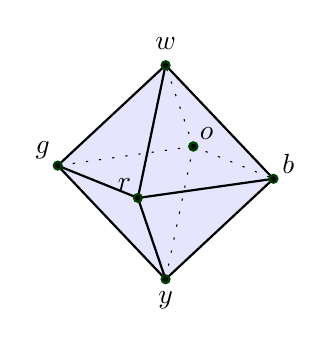
\begin{tikzpicture}%
  [x={(-0.860769cm, -0.121512cm)},
  y={(0.508996cm, -0.205391cm)},
  z={(-0.000053cm, 0.971107cm)},
  scale=1,
  back/.style={loosely dotted, thin},
  edge/.style={black, thick},
  facet/.style={fill=blue!95!black,fill opacity=0.1},
  vertex/.style={inner sep=1pt,circle,draw=green!25!black,fill=black,thick}]
\coordinate (-1, -1, 0) at (-1, -1, 0);
\coordinate (-1, 1, 0) at (-1, 1, 0);
\coordinate (0, 0, -1) at (0, 0, -1);
\coordinate (0, 0, 1) at (0, 0, 1);
\coordinate (1, -1, 0) at (1, -1, 0);
\coordinate (1, 1, 0) at (1, 1, 0);
%% Drawing edges in the back
%%
\draw[edge,back] (-1, -1, 0) -- (-1, 1, 0);
\draw[edge,back] (-1, -1, 0) -- (0, 0, -1.4);
\draw[edge,back] (-1, -1, 0) -- (0, 0, 1.4);
\draw[edge,back] (-1, -1, 0) -- (1, -1, 0);
%% Drawing vertices in the back
%%
\node[vertex] at (-1, -1, 0)     {};
%% Drawing the facets
%%
\fill[facet] (1, 1, 0) -- (0, 0, -1.4) -- (1, -1, 0) -- cycle {};
\fill[facet] (1, 1, 0) -- (0, 0, 1.4) -- (1, -1, 0) -- cycle {};
\fill[facet] (1, 1, 0) -- (-1, 1, 0) -- (0, 0, 1.4) -- cycle {};
\fill[facet] (1, 1, 0) -- (-1, 1, 0) -- (0, 0, -1.4) -- cycle {};
%% Drawing edges in the front
%%
\draw[edge] (-1, 1, 0) -- (0, 0, -1.4);
\draw[edge] (-1, 1, 0) -- (0, 0, 1.4);
\draw[edge] (-1, 1, 0) -- (1, 1, 0);
\draw[edge] (0, 0, -1.4) -- (1, -1, 0);
\draw[edge] (0, 0, -1.4) -- (1, 1, 0);
\draw[edge] (0, 0, 1.4) -- (1, -1, 0);
\draw[edge] (0, 0, 1.4) -- (1, 1, 0);
\draw[edge] (1, -1, 0) -- (1, 1, 0);
%% Drawing the vertices in the front
%%
\begin{scope}[nodes=vertex]
\node[label=above right:\( b \)] at (-1, 1, 0)     {};
\node[label=below:\( y \)] at (0, 0, -1.4)     {};
\node[label=above:\( w \)] at (0, 0, 1.4)     {};
\node[label=above left:\( g \)] at (1, -1, 0)     {};
\node[label=above left:\( r \)] at (1, 1, 0)     {};
\node[label=above right:\( o \)] at (-1, -1, 0)     {};
\end{scope}
\end{tikzpicture}
\caption{The HIT \( \oo \) which has 6 points, 12 1-paths, 8 2-paths.}
\end{figure}

\caption{The Hasse diagram of the simplicial complex \( O \), and a possible realization. The row of singletons in the Hasse diagram is \( O_0 \) and above it are \( O_1 \) and \( O_2 \).}
\label{fig:hasse_octohedron}
\end{figure}

We can realize \( O=[O_0, O_1, O_2] \) as a cellular type \( \oo \).

\begin{mylemma}
\label{lem:octahedron_sphere}
There is an equivalence \( \oo_2\simeq S^2 \).
\end{mylemma}
\begin{myproof}Omitted.\end{myproof}
